\chapter{General Introduction}
\label{chap:introduction}

% NC: This is really good, I know what you mean almost the whole time, my comments are more to polish it up. There's a couple of paragraphs to add but otherwise this won't need a huge amount more work.

%Some quote from GG Simpson
%"Certainly paleontologists have found samples of an extremely small fraction, only, of the earth's extinct species, and even for groups that are most readily preserved and found as fossils they can never expect to find more than a fraction.""
%But I'm not sure, maybe not quote is better.

% NC: It's always fun to have a cheesy quote, but not necessary. That quote isn't really great. FYI Simpson mentions the mammal question in his 1944 book on one of the pages with mammals on it (can't recall which but I was looking in the index at mammals).

%---------------------
%
% GENERAL INTRO - MAKE IT SHORT - TG: this version is a bit long I think, I'll shorten it up (biology letters style) after first round editing.
% 
%---------------------

Today's diversity of living organisms represents an overwhelmingly small fraction of the organisms that have ever existed \citep{novacek1992ext,raup1993extinction}.
Nonetheless, although it is widely accepted that the biodiversity patterns % NC: I don't like using biodiversity twice so close together BUT you need to say what kinds of patterns. Could be curtain patterns for all I know. TG: Ah! I knew I should have done a PhD on curtain patterns. - replaced the first biodiversity above.
we observe today are influenced by evolutionary history \citep{simpson1945,Gingerich1987,archibald2011extinction}, much research focuses solely on living or fossil species separately.
This narrow focus can lead to misinterpretation of macroevolutionary patterns and processes \citep{fritzdiversity2013,benton2015}.
For example, \cite{Wiens2015} suggest that terrestriality is a driver of diversification among living vertebrates, a pattern essentially driven by Aves (birds), Squamata (lizards and snakes) and Mammalia. 
Living crocodilians are also included in the analysis but because they constitute a species poor group \citep[25 species;][]{uetz2010original}, living in only a few types of environments \citep[marine or freshwater;][]{Martin2008}, they only had a marginal effect on the conclusion of this study.
However, extinct crocodilians were much more diverse than present-day species, both in terms of species richness \citep[at least 244 species are reported in][]{Bronzati2015} and the environments they lived in \citep[extinct crocodilians species ranged from fully marine ones to fully terrestrial ones -- including even few tree-dwelling! --][]{stubbs2013}.
Therefore, by not including fossil species, \cite{Wiens2015} conceals the true history of this clade, and thus, potentially biases the conclusions of the study.

Including fossil species not only accounts for groups that were more diverse in the past, it also improves our descriptions of macroevolutionary patterns such as the timing of diversification events \citep[e.g. significantly reducing node age confidence intervals;][]{ronquista2012}, speciation scenarios \citep[e.g. revealing hidden vicariance patterns;][]{Wood01032013} or niche occupancy through time \citep[e.g.][]{pearmanniche2008}.
These studies have led to increasing consensus among evolutionary biologists that we need to combine both living and fossil species in macroevolutionary analyses \citep{jacksonwhat2006,quentaldiversity2010,dietlconservation2011,slaterunifying2013,fritzdiversity2013,benton2015}.

% TG: add croc figure? with/without fossils?
% NC: That would be nice, but not necessary if you're rushed for time. TG: I'll see if I can get a hand on Bronzati's phylogeny. 
% TG: Illustrations (pictures of the crocodiles) - Not entirely convinced
\begin{figure}[!h] 
\centering
    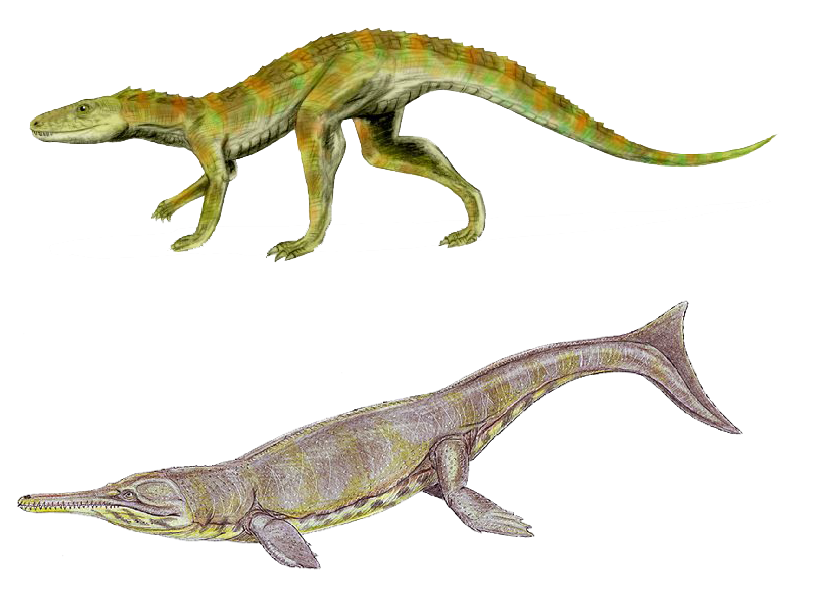
\includegraphics[keepaspectratio=true]{introduction/figures/Crocodilians.pdf}
\caption[Fossil crocodilians]{Two fossil crocodilians. Upper: \textit{Hesperosuchus agilis} (Late Triassic -- 227-208Ma -- image: CC BY 2.5, Nobu Tamura). Lower: \textit{Metriorhynchus superciliosus} (Late Jurassic -- 167-155 Ma -- image: CC BY 3.0, Dmitry Bogdanov)}
\label{fig:intro}
\end{figure}


Testing macroevolutionary hypothesis first requires a phylogenetic tree of the group of interest where the evolutionary patterns can be observed.
Yet, in practice, few studies have actively focused on such a combination and most were published in the last five years \citep[e.g.][]{ronquista2012,slaterphylogenetic2013,Wood01032013,beckancient2014}.
The scarcity of such studies combining living and fossils species is probably due to the fact that palaeontologists and biologists working on living species (i.e. neontologists) %/evolutionary biologists TG: some evolutionary biologists are palaeontologists no? And some neontologists are not evolutionary biologists no (e.g. people looking a TB and badgers)?
use different kinds of data, and different methods, to build their phylogenies.
% NC: You're confusing macroevolution here with tree building. I've tried to be more specific. TG: good point!
Palaeontological phylogenies are generally based on cladistic data from the fossil record (i.e. discrete morphological observations).
Phylogenetic reconstructions then rely on optimality criteria such as maximum parsimony \citep{Hennig1966,felsenstein2004} to resolve the relations among lineages and on stratigraphy to date these trees \citep{GoloboffTNT}.
This allows a direct interpretation of macroevolution in deep time and benefits from recent increased data collection efforts \citep[e.g. 4541 characters in][introducing the term ``phenomics'']{O'Leary08022013} and improvements in tree dating methods \citep[e.g. the \textit{cal3} method from][]{Bapst2014}.
However, palaeontological studies rarely take into account all of living diversity \citep[e.g. only 38 out of 351 living primates are included with 119 fossils in][]{ni2013oldest} and these methods suffer from several biases \citep[e.g. parsimony;][]{wrightbayesian2014}. %TG: or: "(e.g. evolution is not parsimonious; Wright and Hillis 2014)." but that's not exactly what they say, just what they show.

Conversely, neontological studies use the vast amount of available molecular data from living species and probabilistic methods (e.g. Maximum Likelihood or Bayesian) for building phylogenies.
These methods are based on evolutionary models that rely on the differences in DNA to resolve relations among lineages and on some specific fossil occurrence dates for dating the trees \citep[i.e. the molecular clock;][]{zuckerkandl1965}.
There have been extensive improvements in these tree building methods in the last decade in both the evolutionary models \citep[e.g.][]{bapsta2013,stadlerdating2013,heaththe2013} and in how fossils are used to time calibrate the trees \citep{Donoghue2007424,Parham01032012}.
However, this approach uses only the ages of certain fossils instead of all the information available from the fossil record (e.g. species richness, traits, biogeography, etc.).
What we really need to move the field of macroevolution forward are phylogenies containing both living and fossil taxa.

Encouragingly, the last three years have seen many improvements of the Total Evidence method \citep{ronquista2012,slaterphylogenetic2013,Wood01032013,schragocombining2013,beckancient2014,Arcila2015131,Dembo2015}; a method that combines both molecular data from living taxa and morphological data from living and fossil taxa in the same phylogenies.
It was first developed in the nineties \citep{eernissetaxonomic1993} but only recently successfully implemented in user-friendly phylogenetic software \citep{Ronquist2012mrbayes,BEAST2}.
By using all the available neontological and palaeontological data, this method can greatly improve the estimation of divergence events \citep[e.g.][]{ronquista2012}; evolutionary rates \citep[e.g.][]{beckancient2014}; tree topology \citep[e.g.][]{Dembo2015}; trait evolution \citep[e.g.][]{slaterphylogenetic2013} and even speciation processes \citep[e.g.][]{Wood01032013}.

% NC: This needs more here I think, maybe a separate paragraph. Same as we mentioned for the discussion, essentially leading the reader into the thesis and what you're going to discuss for the rest of the intro.
In the following thesis, I explore the Total Evidence method in terms of its benefits and its drawbacks for studying macroevolution.
In the first part of this thesis, I looked on the practical implications of combining paleontological and neontological data by focusing at the effect of missing data on tree topology.
In the second part of this thesis, I used a Total Evidence phylogeny to explore the effect of mass extinctions on morphological evolution, using mammals as an example.

\section{Missing data and the Total Evidence method}
As introduced above, the Total Evidence method seems to be a promising method for combining living and fossil species into macroevolutionary studies.
There is, however, one drawback to this method: because it needs both molecular data for living taxa and morphological data for living and fossil taxa, Total Evidence phylogenies are likely to have a large proportion of missing data.
In chapter \ref{chap:TEM_paper}, I therefore tackle the problem of missing data in Total Evidence matrices.
I perform extensive simulations to test how sensitive topologies inferred from Total Evidence matrices are to missing data in the morphological partition of the matrix, by removing data according to three parameters: (1) the number of living taxa with molecular data but no morphological data; (2) the amount of missing data in the fossil record; and (3) the overall number of morphological characters in the matrix.
I then build phylogenies from the complete matrices, and matrices with varying amounts of missing data, using both Maximum Likelihood and Bayesian inference methods.
Finally, I compare how my missing data parameters and their interactions, as well as the phylogenetic inference method, influence the ability to estimate the correct tree topology.

One of the main conclusions of chapter \ref{chap:TEM_paper} is that to recover accurate topologies, we need as much morphological data for living species as possible.
However, no estimates of the amount of morphological data already coded for living species exist.
Therefore, in chapter \ref{chap:missing_mammals}, I investigate the availability of morphological data in the literature for living mammals.
I download available morphological matrices and count the number of living mammals with available morphological data at three different taxonomic levels (species, genus and family) for each mammalian order.
I then measure whether the missing data are biased toward toward specific clades in each order using community phylogenetics methods \citep{webb2002phylogenies}.


\section{Using Total Evidence phylogenies to ask macroevolutionary questions}
Chapters \ref{chap:TEM_paper} and \ref{chap:missing_mammals} focus on the technical and practical aspect of combining living and fossil taxa in the same phylogenies.
However, another interesting question is how can we use these phylogenies to test interesting macroevolutionary questions.
Until now, only several studies have used Total Evidence phylogenies in macroevolutionary studies \citep[e.g.][]{Wood01032013,slaterphylogenetic2013,beckancient2014,Dembo2015} %TG: I think it's useless to develop these examples since they are described many times above.
yielding to more robust results compared to a classical palaeontological or neontological approach.
Therefore, in the final chapter of my thesis I tackled a classical macroevolutionary question by using a Total Evidence phylogeny. 

One example of an interesting macroevolutionary pattern is the shift in ecologically dominant clades through time due to drastic biotic or abiotic changes (e.g. climate change, mass extinctions, land bridge formations; such as the Great American Biological Interchange).
For example, the Brachiopoda were the dominant shelled filter feeding clade during the Paleozoic (514 to 252 million years ago; Ma) but were replaced by Bivalvia at the end Permian extinction event (252 Ma) so that Bivalvia is now the dominant group (\citealt{Sepkiski1981,CLAPHAM01102006,Liow2015} but see \citealt{Payne22052014}).
This type of replacement pattern has also been observed in other groups such as Formaninifera \citep{Coxall01042006}, Ichthyosauria \citep{thorneresetting2011} and Plesiosauria \citep{bensonfaunal2014} and are often related to competition \citep{brusatte50} or adaptive radiations \citep{Losos2010}.
Another classical example is the ``replacement'' of the dominant non-avian dinosaurs by mammals after the infamous Cretaceous-Paleogene (K-Pg) extinction 66 Mya.
In chapter \ref{chap:STD_paper}, I focus on this example, updating classical analyses using Total Evidence phylogenies and various methodological improvements.

I investigate changes in morphological diversity \citep[or disparity;][]{Wills1994} through time using Total Evidence trees from \cite{slaterphylogenetic2013} and \cite{beckancient2014} to test whether the K-Pg extinction event had an effect on mammalian diversification.
I propose a new approach to describe patterns of disparity through time based on the use of Total Evidence trees.
This approach allows more precision in describing the changes through time as well as more freedom for choosing the underlying models of morphological evolution \citep[e.g. punctuated or gradual;][]{Hunt21042015}.

Finally, in chapter \ref{chap:discussion} I draw together the results from chapters \ref{chap:TEM_paper}, \ref{chap:missing_mammals} and \ref{chap:STD_paper} and discuss how the research in these chapters open new avenues for research.
I then discuss the limitation of my analyses, and suggest improvements for future studies.
I also present some concluding thoughts on the utility of combining palaeontological and neontological research for improving our understanding of macroevolutionary patterns and processes.

%\bibliography{References}